% -*- coding: utf-8 -*-
%  $Description: Author guidelines and sample document in LaTeX 2.09$ 
%
%  $Author: ienne $
%  $Date: 1995/09/15 15:20:59 $
%  $Revision: 1.4 $
%

\documentclass[times, 10pt,twocolumn]{article} 
\usepackage{conf/wscad_ieee}
\usepackage{times}
\usepackage[portuges]{babel}
\usepackage{graphicx,url}
\usepackage[utf8x]{inputenc}

\usepackage{xspace}     
\def\sw{\textit{software}\xspace}
\def\hw{\textit{hardware}\xspace}
\def\kernel{\textit{kernel}\xspace}
\def\hpv{hipervisor\xspace}
\def\mmv{{Monitor de Máquinas Virtuais}\xspace}
\def\para{{paravirtualização}\xspace}
\def\dd{\textit{device}\xspace\textit{drivers}\xspace}


%\documentstyle[times,art10,twocolumn,latex8]{article}

%------------------------------------------------------------------------- 
% take the % away on next line to produce the final camera-ready version 
\pagestyle{empty}

%------------------------------------------------------------------------- 
\begin{document}

\title{Análise Comparativa de Desempenho do Hipervisor Xen: Paravirtualização versus Virtualização Total}

\author{Ronaldo Canofre Mariano dos Santos, Andrea Schwertner Charão\\
    Laboratório de Sistemas de Computação (LSC)\\
    Mestrado em  Ciência da Computação --
    Universidade Federal de Santa Maria (UFSM)\\
	Campus UFSM - 971405-900 -- Santa Maria -- RS -- Brasil\\
    \{canofre,andrea\}@inf.ufsm.br}

\maketitle
\thispagestyle{empty}

\begin{abstract}
Tecnologias de virtualização têm sido amplamente utilizadas em
sistemas computacionais, tanto em nível acadêmico quanto comercial.
O desenvolvimento de novos processadores que implementam o suporte à virtualização
ampliou ainda mais este cenário. Dentre as tecnologias de virtualização atuais,
o \hpv Xen está entre os mais populares e destaca-se por oferecer duas
abordagens distintas: a virtualização total assistida por \hw e
a paravirtualização. Este artigo apresenta uma comparação de desempenho entre
essas abordagens, utilizando Xen e analisando características como acesso a
disco, memória, comunicação de rede e utilização do processador. O resultado 
deste trabalho mostra que a utilização do Xen paravirtualizado apresenta um 
melhor desempenho face ao seu suporte à virtualização total.
\end{abstract}


%------------------------------------------------------------------------- 
\section{Introdução}\label{s:introducao}
%Cenário da Virtualização
Nos últimos anos a virtualização tem sido um tema presente nas diversas áreas da
computação. Sua capacidade de executar vários sistemas operacionais de forma
simultânea sobre um mesmo \hw  possibilita um uso mais eficiente dos recursos
disponíveis, uma melhor gerenciabilidade do ambiente, compatibilidade de \sw,
flexibilidade e mais segurança devido ao isolamento de falhas, dentre outras 
vantagens.

Para o uso da virtualização, diversos métodos e ferramentas têm sido propostas,
analisadas e utilizadas, fazendo com que a escolha de uma destas soluções não seja
trivial. Dentre as ferramentas existentes, soluções proprietárias como 
VMWare~\cite{vmware}, ou \textit{open source} como Xen~\cite{xen}, OpenVZ~\cite{openvz}
e KVM~\cite{kvmwiki}, vêm ganhando uma atenção considerável e têm sido amplamente 
utilizadas e comparadas atualmente~\cite{xenopenvz,cappello}, 
sendo também alvos de análises de desempenho~\cite{urschei07}. 

A ferramenta Xen é uma das soluções mais populares e oferece duas abordagens distintas
de virtualização, que exigem modificações no núcleo do sistema hospedado 
(paravirtualização) ou recriam em \sw toda a estrutura de \hw (virtualização 
total, do inglês \textit{full virtualization}). Ambas as formas de implementação inserem
impactos distintos no desempenho de operações básicas do sistema, como acesso a disco, 
memória, comunicação de rede e  utilização do processador (CPU).

Com o desenvolvimento de extensões para arquitetura x86 pela AMD e Intel, 
culminando com a inclusão de novas tecnologias (Pacifica e Vanderpoll respectivamente) 
em seus processadores, tornou-se possível realizar a virtualização total sem a 
necessidade de replicar todos os componentes físicos da máquina real. Isso ocorre 
porque estes processadores oferecem suporte nativo a virtualização, permitindo 
que sistemas hospedados sejam executados como processos, diretamente sobre o \hw. 

%Objetivos e justificativa do trabalho
Neste trabalho, tem-se como objetivo quantificar o impacto da paravirtualização 
e da virtualização total, com suporte assistido por \hw, sobre o desempenho de um 
sistema utilizando Xen. Para isso, utilizam-se \textit{benchmarks} para avaliar o
desempenho de rede,  processador, disco e memória em uma arquitetura com 
tecnologia Intel VT. 

%Seções
O restante deste artigo está organizado como segue: na Seção \ref{s:virtualizacao},
expõe-se os conceitos gerais sobre virtualização e as tecnologias existentes. Na 
Seção \ref{s:mmv_xen}, abordam-se as principais características do \hpv Xen e as 
formas como ele implementa o acesso aos dispositivos físicos. Na Seção \ref{s:analise},
apresenta-se a metodologia e as ferramentas utilizadas. Na Seção \ref{s:res} são 
apresentados e discutidos os resultados obtidos, constituindo a principal contribuição 
deste trabalho. Por fim, na Seção \ref{s:fim}, são apresentadas as considerações finais sobre o trabalho.


%------------------------------------------------------------------------- 
\section{Tecnologias de Virtualização}\label{s:virtualizacao}
%Breve relato sobre virtualização
No final dos anos 50 e início dos 60 se estabelecia um novo conceito de utilização de
máquinas de grande porte, com o emprego de uma técnica que possibilitava o 
compartilhamento de um mesmo \hw por diversas Máquinas Virtuais (MV).

De modo geral, a técnica de virtualização consiste na inserção de uma camada extra de \sw 
denominada Monitor de Máquinas Virtuais (MMV) ou \hpv, entre o sistema físico e o 
sistema operacional, podendo ou não contar com um suporte a virtualização em \hw. 

Assim, torna-se possível a execução de diversos sistemas operacionais 
de forma independente, cujos acessos aos dispositivos físicos são controlados por 
esta camada extra de \sw, proporcionando características como confiabilidade, 
flexibilidade, gerenciabilidade e um bom isolamento de falhas~\cite{goldberg}. 

%Técnicas de virtualização
Para realizar a execução de um ou vários  SO's sobre um mesmo \hw, o MMV necessita 
utilizar-se de alguma técnica que permita a ele fornecer ao SO convidado as 
características e funcionalidades necessárias para que o mesmo execute~\cite{mve}.
Nas seções a seguir são abordadas duas implementações diferentes de monitores
e o suporte oferecido pelos processadores Intel e AMD. 

\subsection{Paravirtualização}
Em arquiteturas semelhantes à IA-32, o MMV não pode interceptar algumas instruções 
geradas pela MV, permitindo assim que esta execute com um maior nível de privilégio. 
Dessa forma, visando possibilitar a virtualização nessas arquiteturas e buscando um 
melhor desempenho na execução dos sistemas convidados~\cite{tg-arthur}, propôs-se o 
uso da paravirtualização.

Nesta técnica são realizadas algumas modificações no núcleo dos SO's convidados e 
hospedeiro, para que possam executar em paralelo contornando estas limitações
~\cite{youseff2006phs}. As modificações realizadas no \hpv resultam em uma interface 
de \hw virtual similar ao \hw real, possibilitando uma melhor interação entre MV e 
MMV, resultando em um menor impacto no desempenho. O principal exemplo de utilização 
é a ferramenta Xen. 

\subsection{Virtualização Total}
Alguns sistemas operacionais não permitem as alterações necessárias para rodar em 
um ambiente paravirtualizado, sendo preciso executarem sobre uma réplica fiel
da arquitetura para qual foram projetados. 

Para tais sistemas, pode-se optar pela técnica de virtualização total, onde o \hpv
replica virtualmente toda a arquitetura necessária. No entanto a recriação de uma 
cópia idêntica do sistema físico acaba inserindo uma maior sobrecarga, conforme
já  verificado em diversos trabalhos~\cite{barham}. 

As ferramentas VMWare Server e Virtual Box~\cite{vbox} são os exemplos mais comuns  
que implementam essa abordagem, executada sobre um sistema hospedeiro. Os monitores
Xen e VMWare ESX, se apoiados por um suporte à virtualização fornecido pelo processador, 
podem executar diretamente sobre o \hw oferecendo virtualização total.
% Esse suporte é abordado na Seção \ref{s:hvm} a seguir.

\subsection{HVM - \textit{Hardware Virtual Machine}}\label{s:hvm}
O suporte a virtualização nativo no \hw, necessário para construção de monitores
eficientes, encontrava-se presente somente em computadores de grande porte, como os
\textit{mainframes}. Atualmente, esse suporte foi disponibilizado nos processadores
Intel e AMD, através de tecnologias denominadas respectivamente de IVT \textit{Intel 
Virtualization Tecnology} ou AMD-V \textit{AMD Virtualization}.

O suporte oferecido por estas tecnologias executa cada máquina virtual como um 
processo independente, diminuindo a necessidade de interrupções constantes do MMV.
Ambas as tecnologias definem dois modos de execução, o modo \textit{root} utilizado 
pelo monitor e que possui todos os privilégios de operação e o modo \textit{non-root},
com os privilégios necessários para que a MV execute sem saber que está sendo 
virtualizada ao mesmo tempo que possa ser controlada pelo \hpv~\cite{intel}. 
%Interrupções e instruções mais sensíveis podem provocar a troca do modo de execução 
%de uma máquina virtual fazendo com que o MMV assuma o controle.

Essa tecnologia oferece vantagens como a execução de um MMV mais simples e com menos 
responsabilidades, não sendo necessário o compartilhamento do espaço de endereçamento
de memória com as MV's, resultando em uma utilização mais eficaz da mesma. Ainda 
possibilita a virtualização das interrupções, uma transição mais eficiente entre 
os modos de operação e acesso completo do monitor ao estado da execução~\cite{tg-gilberto}. 

 
%------------------------------------------------------------------------- 
\section{\mmv Xen}\label{s:mmv_xen}
O Xen é um MMV de código aberto que suporta  arquiteturas como IA-32 e AMD64.
Implementando originalmente a técnica de paravirtualização, a partir da versão 3.0 
passou a oferecer também a virtualização total, desde que executado sobre um \hw HVM.
A arquitetura Xen segue uma estrutura de 4 anéis, sendo o anel 0 o nível mais baixo, 
e o anel 3 o mais alto e menos privilegiado.

Quando executa de forma paravirtualizada, o \hpv Xen, o \kernel e as aplicações, 
executam respectivamente nos anéis 0, 1 e 3, como pode ser visto na Figura 
\ref{fig:aneis} (a). Desta forma o monitor tem maior privilégio de execução e 
controla todas as chamadas de sistema e interrupções da MV. Embora sejam necessárias 
algumas modificações no núcleo do sistema, essa abordagem demonstra um desempenho 
superior quando comparada à virtualização total. 

\begin{figure}[!htb]
\centering
\resizebox{8cm}{!}{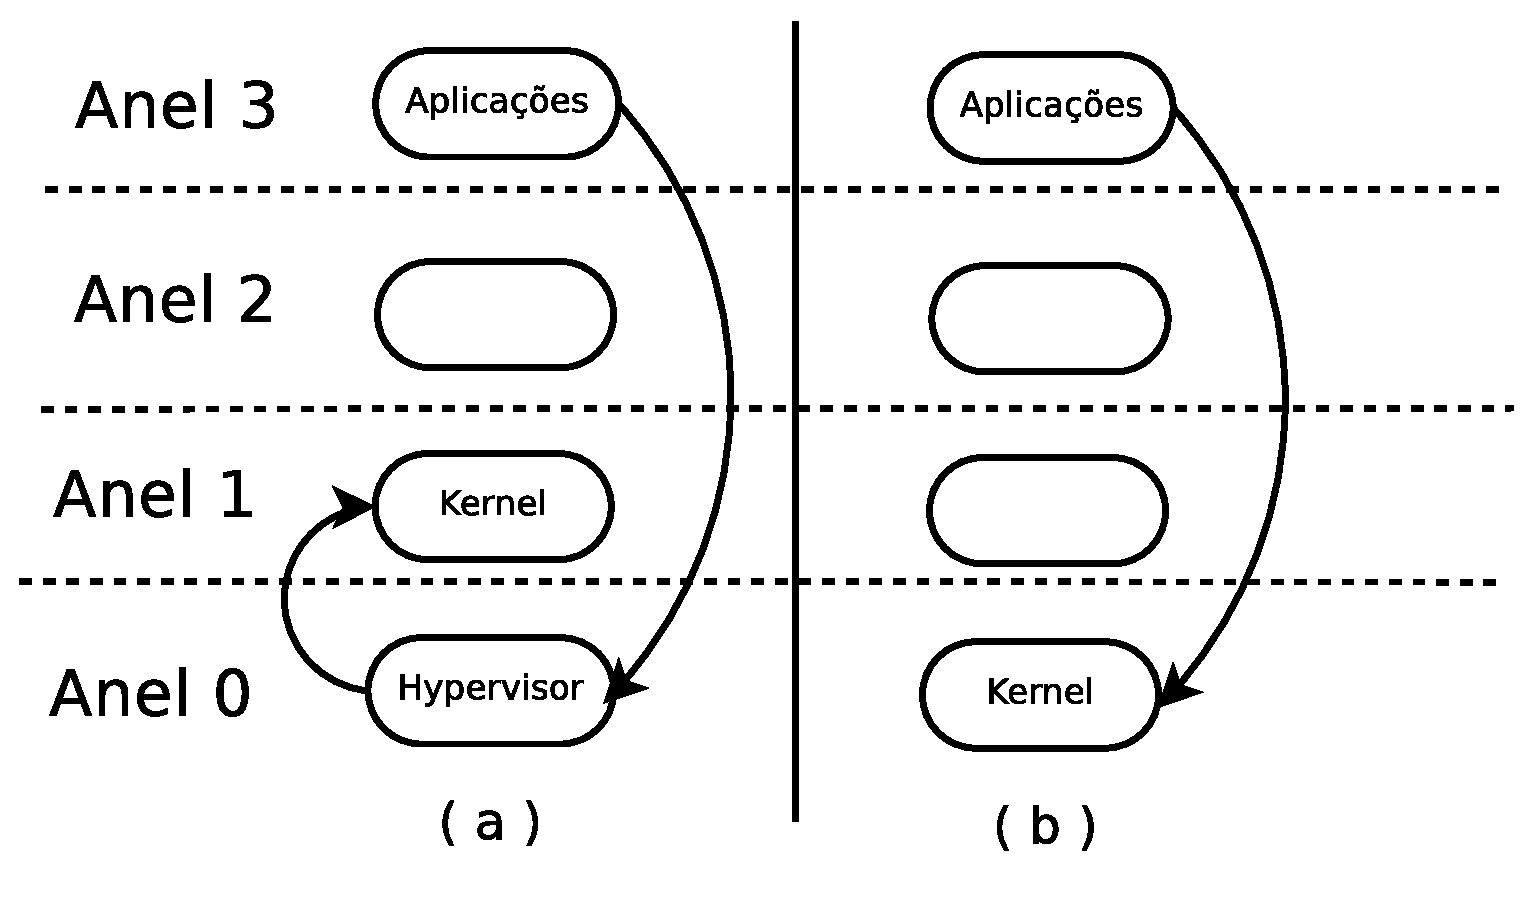
\includegraphics{img/aneis.eps}}
\caption{Organização da arquitetura utilizada pelo MMV Xen}
\label{fig:aneis}
\end{figure}

No entanto, levando em consideração o suporte atual fornecido pelas arquiteturas 
mencionadas anteriormente, o \kernel e as aplicações passam a executar nos anéis 0 e 3 
respectivamente, conforme a Figura \ref{fig:aneis} (b), fazendo com que as aplicações 
passem a ter acesso direto ao núcleo, eliminando a interferência constante necessária 
do monitor para traduzir chamadas de sistemas e interrupções~\cite{xenhpv}. 

Dessa forma torna-se possível através do MMV Xen, virtualizar aplicações que não 
permitem que seu código seja modificado. A utilização desta técnica já foi alvo
de análises e comparações, mostrando que WMWare ESX 3.0.1 e Xen 3.2, ambos
oferecendo virtualização total, apresentaram desempenhos semelhantes~\cite{comparacao,
xenbr}. 

Embora este suporte em \hw simplifique o MMV, ele não o elimina, o que faz com que o
Xen gerencie de formas distintas o acesso a dispositivos e controle das máquinas virtuais,
de acordo com a tecnologia adotada. A seguir será abordada a forma de implementação 
dos dispositivos foco deste trabalho, utilizada pelo Xen.

Em máquinas paravirtualizadas (PVM), a implementação de acesso a disco e dispositivos
de rede é realizada com a utilização de \dd especiais que exportam e compartilham os
recursos com os domínios. Cada domínio (DomU) utiliza-se de um \textit{frontend driver}
para se comunicar com o \textit{backend} do domínio zero (Dom0), que  acessa 
diretamente os dispositivos físicos. Nos domínios totalmente virtualizados (HVM), 
estes dispositivos são emulados e o acesso é realizado com o auxílio de um 
\textit{daemon} Qemu no Dom0, e um \textit{firmware} virtual do Xen que simulam o 
acesso a estes dispositivos~\cite{arqxen}, o que tende a inserir uma maior 
sobrecarga  no desempenho destes dispositivos.

%%%%%%%%%%%%%%%%%%%%%Original
%Em máquinas paravirtualizadas (PVM), a implementação de acesso a disco e dispositivos
%de rede se dá por dois \textit{drivers} instalados no domínio zero (Dom0), que 
%gerenciam as solicitações de acesso aos dispositivos físicos oriundas dos respectivos 
%\textit{drivers} localizados nas MV's. Nos domínios totalmente virtualizados (HVM), 
%estes dispositivos são emulados e o acesso é realizado com o auxílio de um 
%\textit{daemon} Qemu no Dom0, e um \textit{firmware} virtual do Xen que simulam o 
%acesso a estes dispositivos~\cite{arqxen}, o que tende a inserir uma maior 
%sobrecarga  no desempenho destes dispositivos.

A virtualização de memória em domínios paravirtualizados é obtida através de um
mapeamento estático da mesma realizado pelo MMV, reservando uma porção de memória
para cada MV, fazendo com que cada domínio acesse somente a sua região mapeada. A 
diferença nos domínios HVM consiste em funções adicionais no processador e controlador
de memória que permitem um acesso mais direto a mesma. 

%%%%%%%%% Original
%Para realizar a virtualização de memória, o MMV mapeia estaticamente uma porção da
%mesma para cada MV, de forma que um domínio não tenha acesso à região de memória do 
%outro. Essa implementação ocorre tanto para máquinas HVM como PVM.  

Por fim, a utilização dos recursos de CPU em domínios PVM é feita através da 
interceptação do conjunto de instruções pelo monitor, que executa em um nível 
mais privilegiado e devolve para o domínio, ao passo que em máquinas HVM, o 
acesso se dá na maioria das vezes diretamente ao processador, sendo interferido 
pelo MMV somente nos casos em que as instruções possam prejudicar ou danificar o sistema. 


%------------------------------------------------------------------------- 
\section{Análise Comparativa}\label{s:analise}
Os testes realizados têm como principal objetivo analisar o desempenho do acesso a 
disco, memória, utilização de CPU e comunicação de rede face às técnicas de 
virtualização implementadas pelo MMV Xen. O ambiente de testes foi configurado de 
três formas: sem virtualização, com virtualização total e com paravirtualização, para 
qual foi desabilitado o suporte provido pelo processador. Em todos os testes foi 
criada apenas uma MV em cada máquina e para a análise de rede, os testes foram 
realizados sobre duas máquinas idênticas interconectadas.

As máquinas utilizadas foram dois servidores Intel x86\_64 SGI Altix XE 210, com CPU
Intel Xeon E5335 2.0 GHz e memória de 8GB. O \kernel utilizado para os testes foi 
o 2.6.20, com Xen versão 3.2.0. A conexão entres as máquinas  foi realizada através
de um \textit{switch} Ethernet de 100 Mbps e os testes foram realizados em uma rede
isolada, proporcionando um ambiente controlado, evitando influências de tráfego 
adicional. 

Os \textit{benchmarks} utilizados para cada análise foram escolhidos devido a 
sua ampla utilização em avaliações de desempenho, sendo os mesmos abordados nas 
seções a seguir. Buscando um resultado mais confiável, realizaram-se 10 execuções
para todos os valores obtidos, calculando-se a média aritmética, 
o desvio padrão e o coeficiente de variação. 

%rede - netperf
Para a análise de desempenho da comunicação de rede, escolheu-se o \textit{benchmark}
Netperf~\cite{netperf}, que permite realizar diversos testes através das modificações 
de seus parâmetros e métricas. Nos testes realizados foram alterados os tamanhos das
mensagens utilizando como métrica a taxa de transferência, através de comunicações
Request-Response com os protocolos TCP e UDP. Os grupos de tamanhos de mensagens 
utilizados foram classificados como pequenas (até 512 bytes), médias (até 512 Kbytes) 
e grandes (até 45 Mbytes), tendo sido estes tamanhos escolhidos por representarem 
desde serviços básicos de rede até transferências de arquivos.

%Memória - STREAM
O \textit{benchmark} STREAM~\cite{stream} é utilizado na análise de largura de banda 
de memória. Este programa mede o desempenho através de quatro testes de 
processamento vetorial, onde os vetores são aumentados para eliminar o reuso de cache
e descrever os resultados em termos de largura de banda contínua. Os resultados 
obtidos com este teste são:

\begin{itemize}
	\item \textit{Copy}: analisa a taxa de transferência através da operação 
		a(i) = b(i);
	\item \textit{Scale}: realiza operações aritméticas simples através da
		operação a(i) = q*b(i);
	\item \textit{Add}: acrescenta um terceiro operando para permitir que  
		múltiplas operações de load/store sejam testadas em máquinas vetoriais, 
		através da operação a(i) = b(i) + c(i);
	\item \textit{Triad}: múltiplas operações de soma e multiplicação através da
		operação a(i) = b(i) + q*c(i);
\end{itemize}

%Disco - dd
Para realizar as medições de acesso ao disco, optou-se por uma ferramenta nativa do
SO Linux, o dd, que realiza cópias de arquivos, de entrada padrão para uma saída 
padrão, podendo utilizar diferentes tamanhos de blocos de entrada e saída.
A execução do dd retorna dois valores, a taxa de transferência de dados entre os 
arquivos em Mbytes/s e o tempo dessa operação em segundos. 

%cpu - linpack
A análise de utilização de CPU foi realizada com a utilização do Linpac-pc, que contém 
dois conjuntos de rotinas: um para decomposição de matrizes e outro para resolver 
o sistema de equações lineares resultantes da decomposição. O mesmo foi escolhido 
devido à métrica utilizada e a sua ampla utilização em testes de desempenho.
Os testes foram realizados com matrizes de tamanho 100 x 100, utilizando precisão simples,
sendo a saída deste \textit{benchmark} o resultado das operações de ponto flutuante 
sobre as matrizes, em Mflops.


%------------------------------------------------------------------------- 
\section {Resultados Obtidos}\label{s:res}
Ao longo desta Seção apresenta-se os resultados obtidos durante a execução 
dos \textit{benchmarks} escolhidos, realizando uma análise comparativa entre
as abordagens utilizadas. Na Tabela \ref{t:cv}, são apresentados todos os 
coeficientes de variação (CV) máximos obtidos em cada grupo de testes, onde
as siglas P, M e G representam os tamanhos dos grupos de mensagens (pequenas,
médias e grandes respectivamente), e as letras C, S, A e T, as iniciais de cada
teste de memória (\textit{Copy}, \textit{Scale}, \textit{Add} e \textit{Triad} 
respectivamente).

\begin{table}[ht]
\centering
\caption{Coeficientes de Variação}
\label{t:cv}
    \begin{tabular}{l|c|c|c}
    \hline Teste&	PVM& HVM& SV\\
    \hline TCP P&	8,2 X $10^{-2}$&    3,73 X $10^{-2}$&	13,76 x $10^{-2}$ \\
    \hline TCP M&	1,06 X $10^{-2}$&   17,38 X $10^{-2}$&	1,62 x $10^{-2}$ \\
    \hline TCP G&	1,49 X $10^{-2}$&    7,38 X $10^{-2}$&	1,53 x $10^{-2}$ \\
    \hline UDP P&	0,11&		     0,01&		0,12 \\
    \hline UDP M&	0,02&		     0,6&		0,17 \\
    \hline Disco&	0,37&		     0,06&		0,26\\
%    \hline Disco (s&)	& & \\
    \hline Mem C&	3,26 X $10^{-2}$&    1,27 X $10^{-2}$&	1,71 X $10^{-2}$\\
    \hline Mem S&	3,31 X $10^{-2}$&    1,38 X $10^{-2}$&	1,37 X $10^{-2}$\\
    \hline Mem A&	2,54 X $10^{-2}$&    0,83 X $10^{-2}$&	0,94 X $10^{-2}$\\
    \hline Mem T&	2,48 X $10^{-2}$&    0,75 X $10^{-2}$&	0,42 X $10^{-2}$\\
    \hline CPU&		4,42 X $10^{-4}$&    8,92 x $10^{-2}$&  4,52 x $10^{-2}$\\
    \end{tabular}
\end{table}


\subsection{Desempenho de Rede}
Nos gráficos das Figuras \ref{fig:tcpp} e \ref{fig:tcpm} tem-se os resultados das 
transferências de mensagens consideradas de tamanho pequeno e médio, obtidas com 
o protocolo TCP. Estes tamanhos são considerados comuns em serviços básicos de rede, 
o que justifica a sua escolha. 

\begin{figure}[!htb]
\centering
\resizebox{9.1cm}{!}{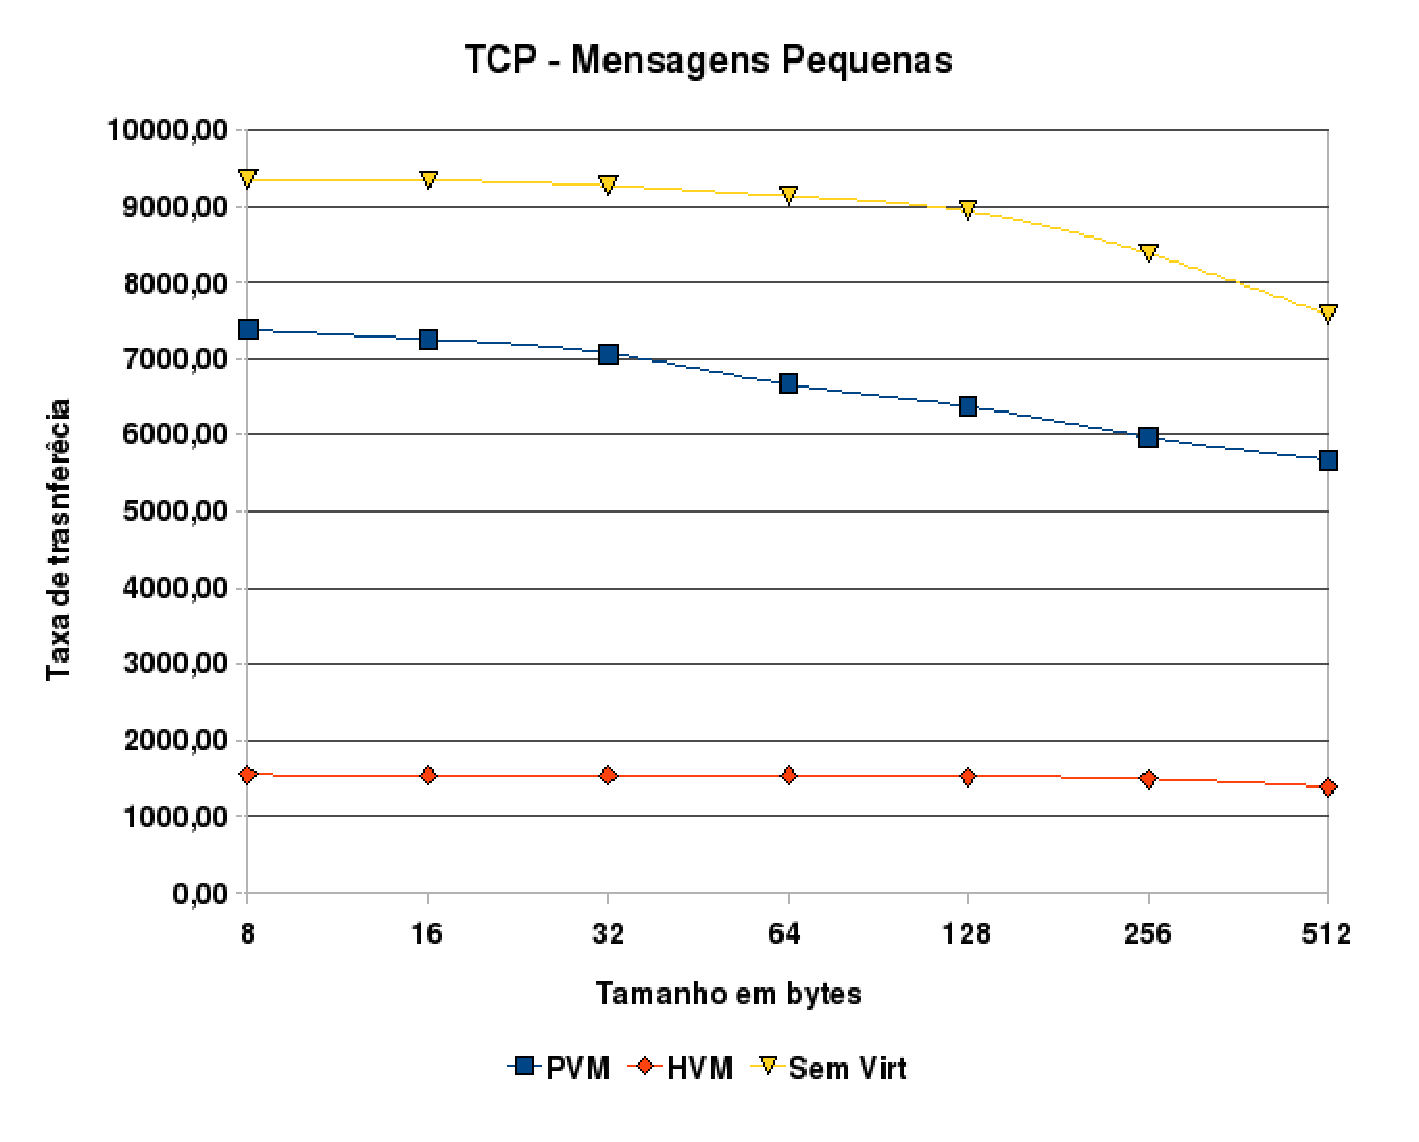
\includegraphics{img/tcp_p.eps}}
\caption{Taxas de transferência TCP, com mensagens pequenas, até 512 bytes}
\label{fig:tcpp}
\end{figure}

No grupo de mensagens com tamanho até 512 bytes, nota-se  o visível impacto da 
virtualização sobre o desempenho da rede, independente da técnica utilizada. No 
grupo de mensagens 512 Mbytes, o impacto apresentado foi  mais acentuado na 
técnica de virtualização total, tendo a paravirtualização um desempenho relativamente 
superior, aproximando-se do desempenho da máquina real a medida que o tamanho das 
mensagens aumenta.
% Para esse grupo

\begin{figure}[!htb]
\centering
\resizebox{8.7cm}{!}{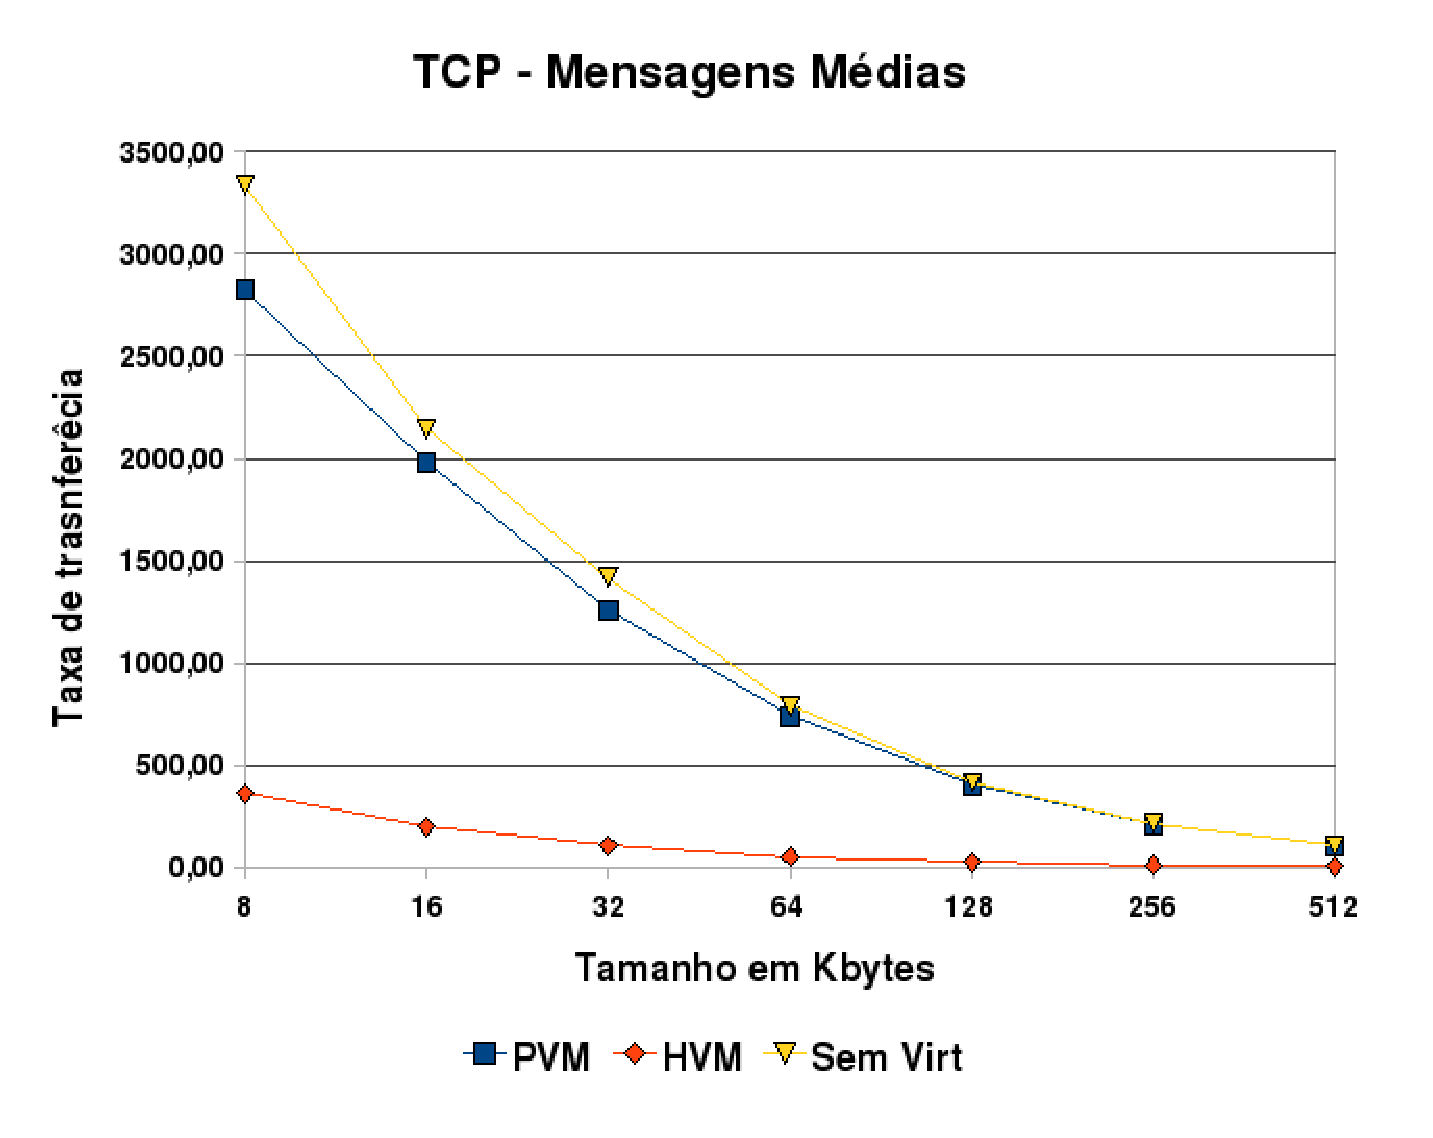
\includegraphics{img/tcp_m.eps}}
\caption{Taxas de transferência TCP, com mensagens médias, até 512 Kbytes}
\label{fig:tcpm}
\end{figure}

Os resultados das transferências com mensagens de tamanho grande com a utilização do
protocolo TCP são mostrados na Figura \ref{fig:tcpg}, onde é possível notar 
que as mensagens atingem no máximo 45 Mbytes. Esta limitação foi imposta pelo 
\textit{benchmark} Netperf, o qual não permite o envio de mensagens maiores que 
50 Mbytes em média.

A escolha destes tamanhos de mensagens se justifica pelo seu uso em aplicações que 
realizam transferências de arquivos. Neste grupo de mensagens, as máquinas HVM 
mantêm seu desempenho inferior ao passo que as máquinas PVM apresentam um desempenho 
eficiente, praticamente igualando-se ao da máquina real.

\begin{figure}[!htb]
\centering
\resizebox{8.7cm}{!}{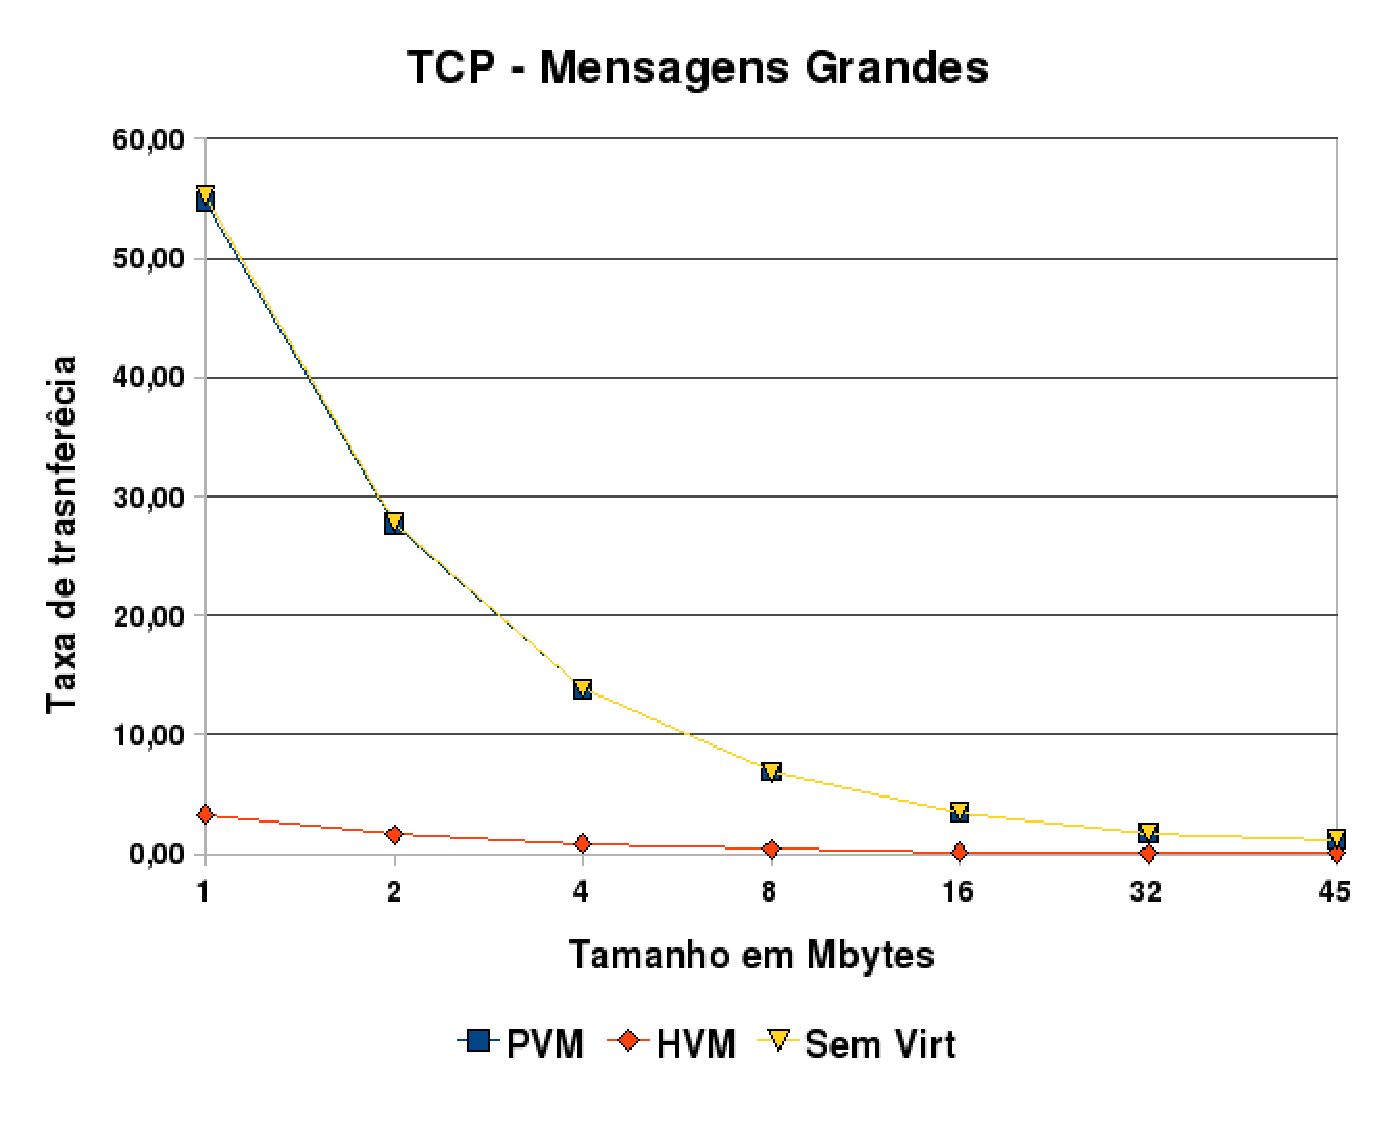
\includegraphics{img/tcp_g.eps}}
\caption{Taxas de transferência TCP, com mensagens grandes, até 45 Mbytes}
\label{fig:tcpg}
\end{figure}

A análise realizada com o protocolo UDP é apresentada nas Figuras \ref{fig:udpp} e 
\ref{fig:udpm} a seguir, onde são analisadas mensagens de dois grupos de tamanho,
pequeno e médio. A realização de testes com um grupo de mensagens maiores que
62 Kbytes, não foi possível devido as limitações impostas pelo \textit{benchmark} 
utilizado.
%A não realização de testes com mensagens superiores a 62 Kbytes deve-se também a limitações impostas pelo próprio \textit{benchmark} adotado.

\begin{figure}[!htb]
\centering
\resizebox{9.1cm}{!}{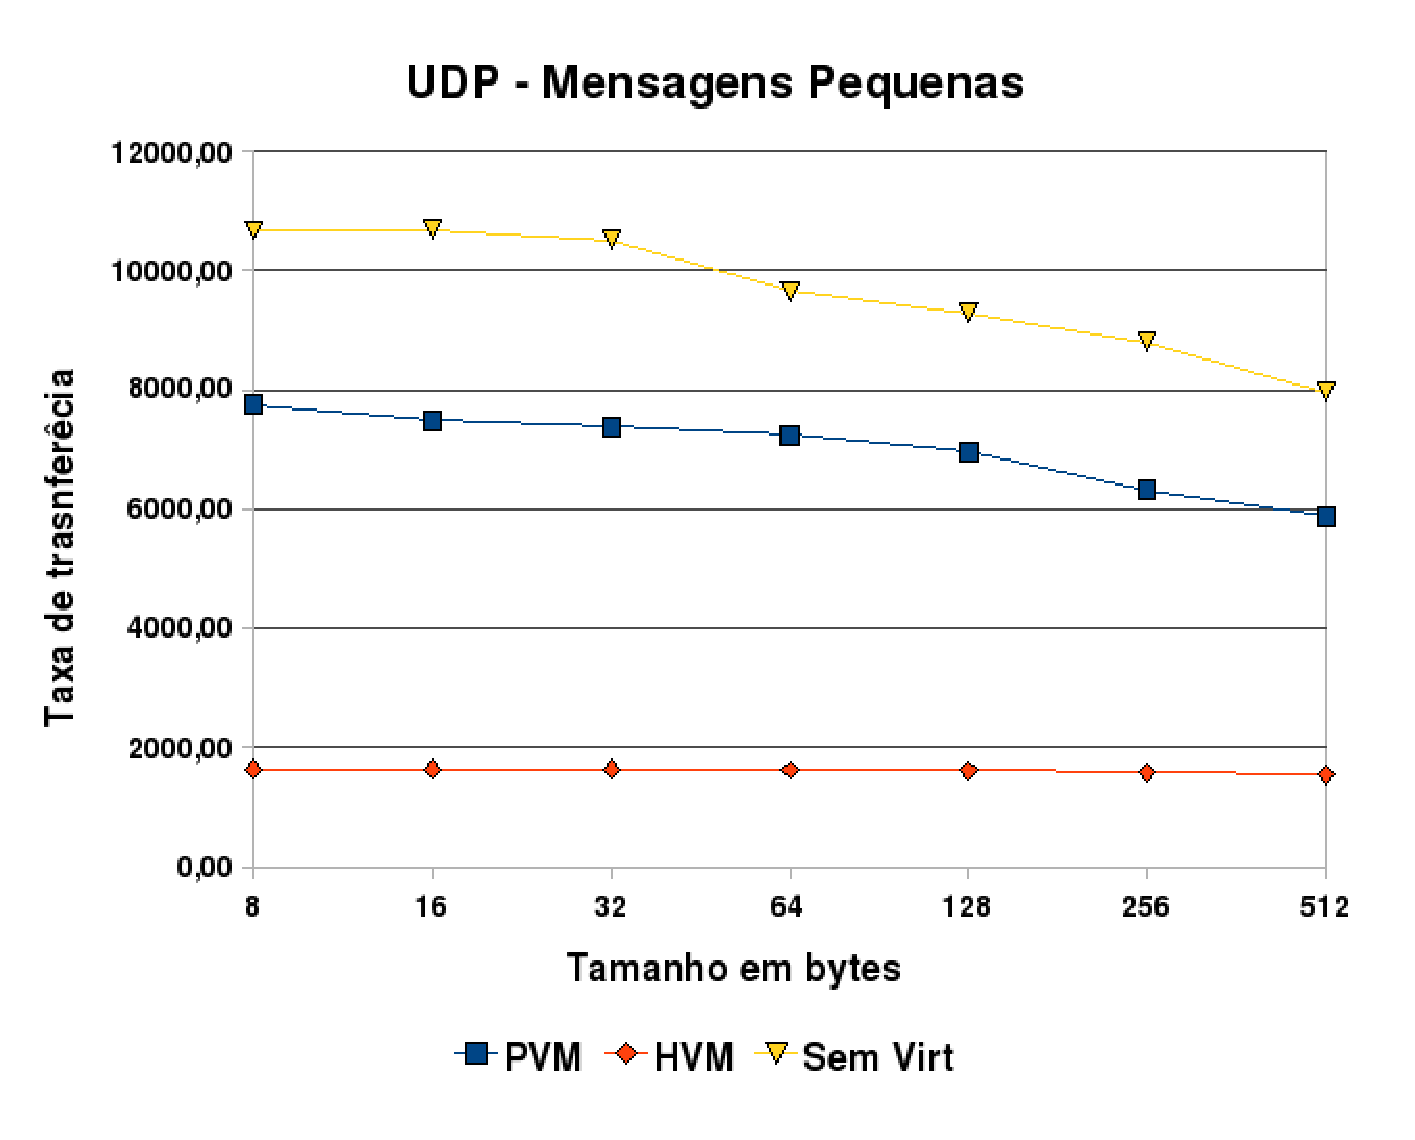
\includegraphics{img/udp_p.eps}}
\caption{Taxa de transferência UDP, com mensagens pequenas, até 512 bytes}
\label{fig:udpp}
\end{figure}

Na transferência de mensagens UDP até 512 bytes é possível observar o impacto de ambas
as tecnologias utilizadas, sendo mais acentuada nas máquinas HVM. Com o 
aumento do tamanho das mensagens até 62 Mbytes, ocorre uma diminuição da 
sobrecarga imposta pelas máquinas PVM, aproximando-se do desempenho do sistema 
hospedeiro, conforme já observado em outras análises~\cite{urschei07,errc2007}. 
É possível observar que da mesma forma que com o protocolo TCP, à medida que aumentam 
os tamanhos das mensagens do protocolo UDP, a diferença de desempenho diminui.

\begin{figure}[!htb]
\centering
\resizebox{8.7cm}{!}{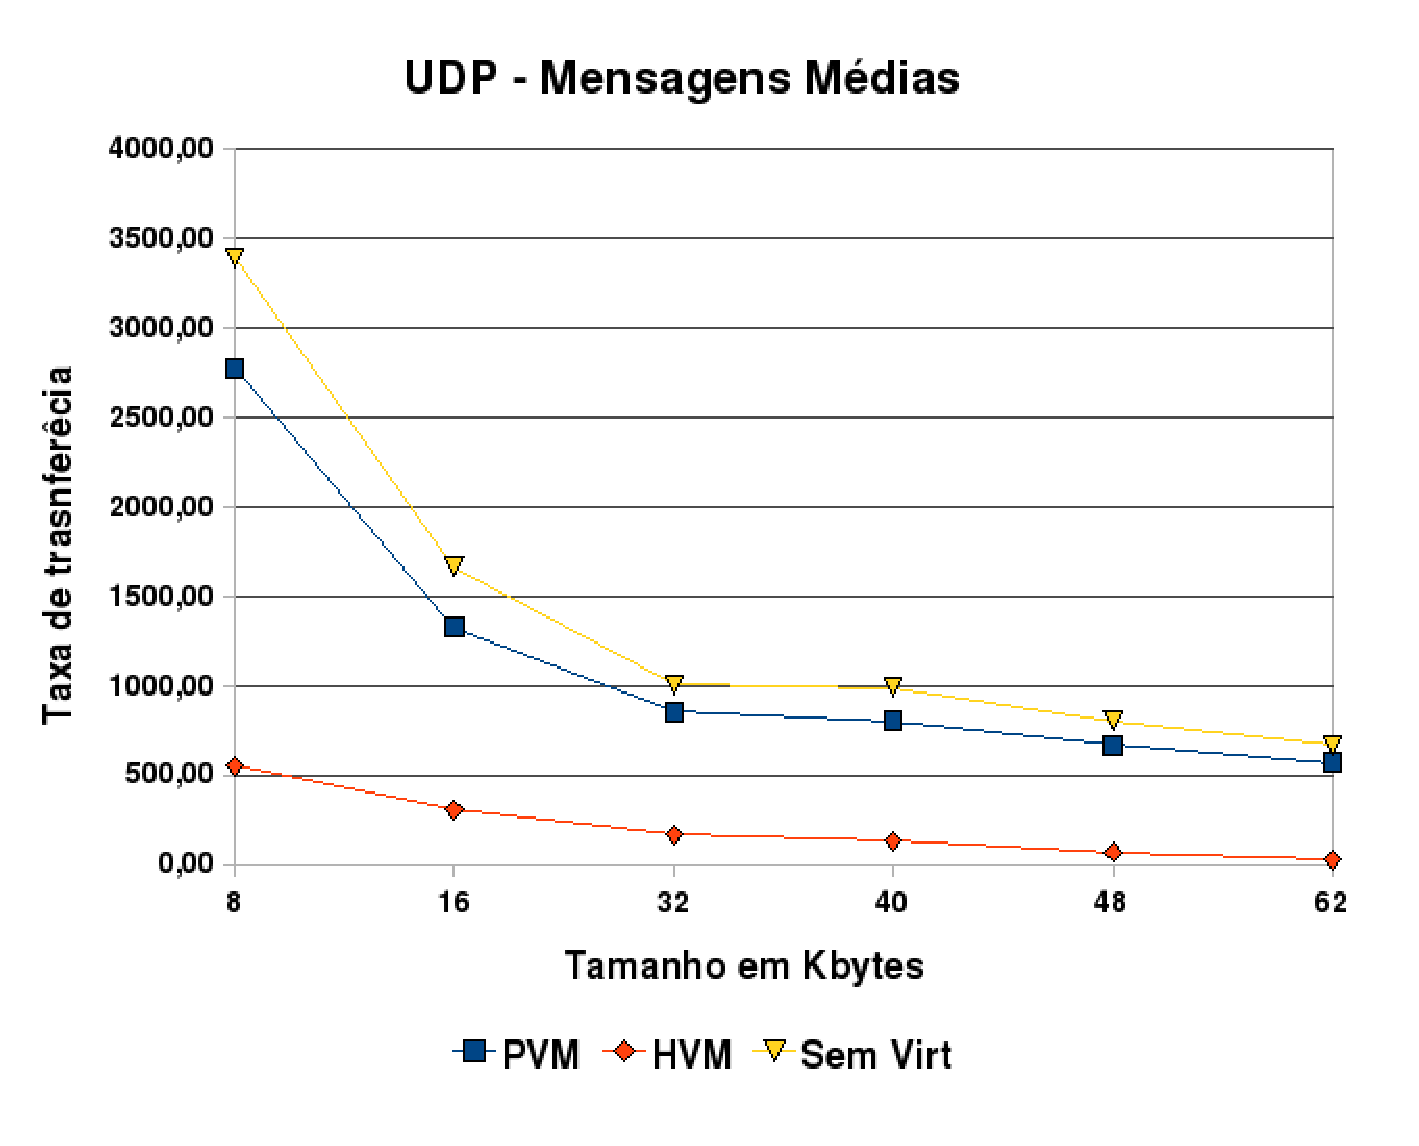
\includegraphics{img/udp_m.eps}}
\caption{Taxa de transferência UDP, com mensagens médias, até 62 Mbytes}
\label{fig:udpm}
\end{figure}

%EXPLICAR O POR QUE DA SUPERIORIDADE, TEM NUM TG
\subsection{Desempenho de memória}
O gráfico mostrado na Figura \ref{fig:mem}  expõe as taxas obtidas nos testes de 
memória. Através deste pode-se observar uma  superioridade no desempenho das máquinas 
HVM em relação as PVM, mas de maneira geral, o desempenho da memória não sofre 
muito impacto independentemente da técnica de virtualização empregada. 

\begin{figure}[!htb]
\centering
\resizebox{8.7cm}{!}{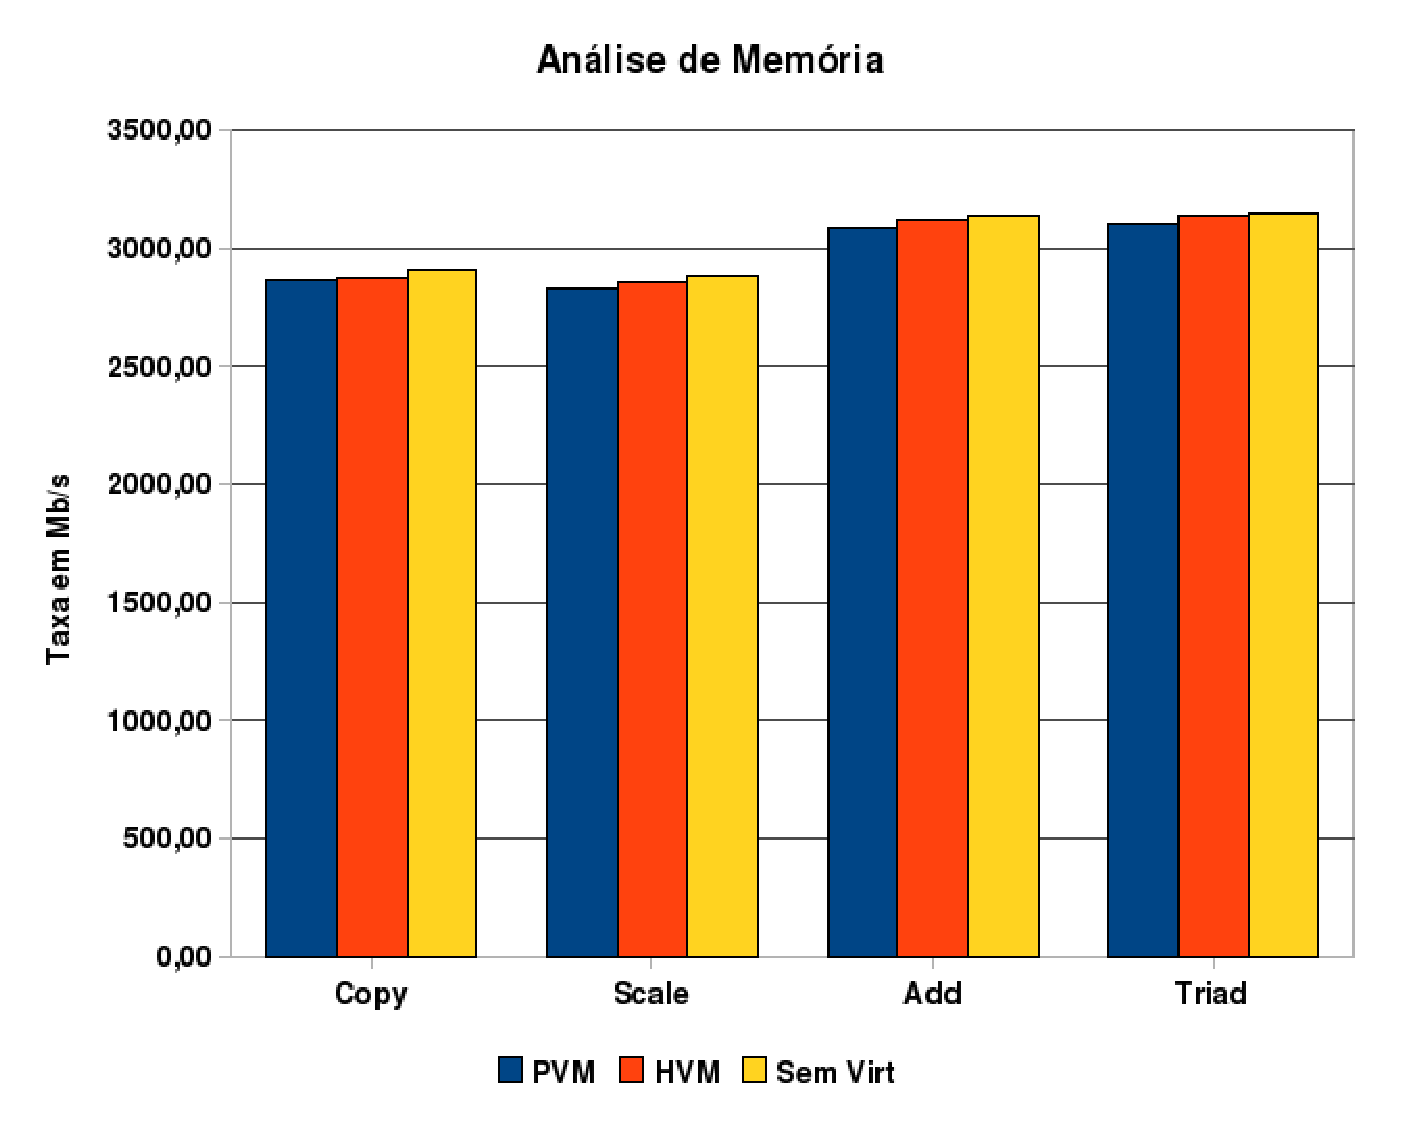
\includegraphics{img/memoria.eps}}
\caption{Taxa de análise de memória em Mbytes/s}
\label{fig:mem}
\end{figure}

\subsection{Desempenho de Disco}
A seguir, são analisados os resultados obtidos com o programa dd,
mantendo seu tamanho de blocos padrão (512 bytes), modificando apenas os tamanhos dos 
arquivos a serem criados. Os testes realizados envolveram arquivos de 6 tamanhos 
distintos, variando entre 128 Mbytes e 4 Gbytes, os quais foram escolhidos devido a 
englobarem tamanhos de arquivos normalmente utilizados em diversas aplicações.

A taxa de transferência para cada tamanho de arquivo obtida é mostrada na 
Figura \ref{fig:disco_t}, onde observa-se de forma geral que o desempenho da máquina
HVM é inferior ao da máquina PVM.  Mais detalhadamente, para arquivos menores, 
a sobrecarga inserida pela virtualização total é bem elevado ao passo que o 
da paravirtualização é relativamente baixo. À medida que o tamanho dos arquivos vai 
aumentando, a máquina PVM aproxima-se das taxas da máquina HVM, apresentando um 
relativo distanciamento do desempenho sem virtualização. 

\begin{figure}[!htb]
\centering
\resizebox{8.7cm}{!}{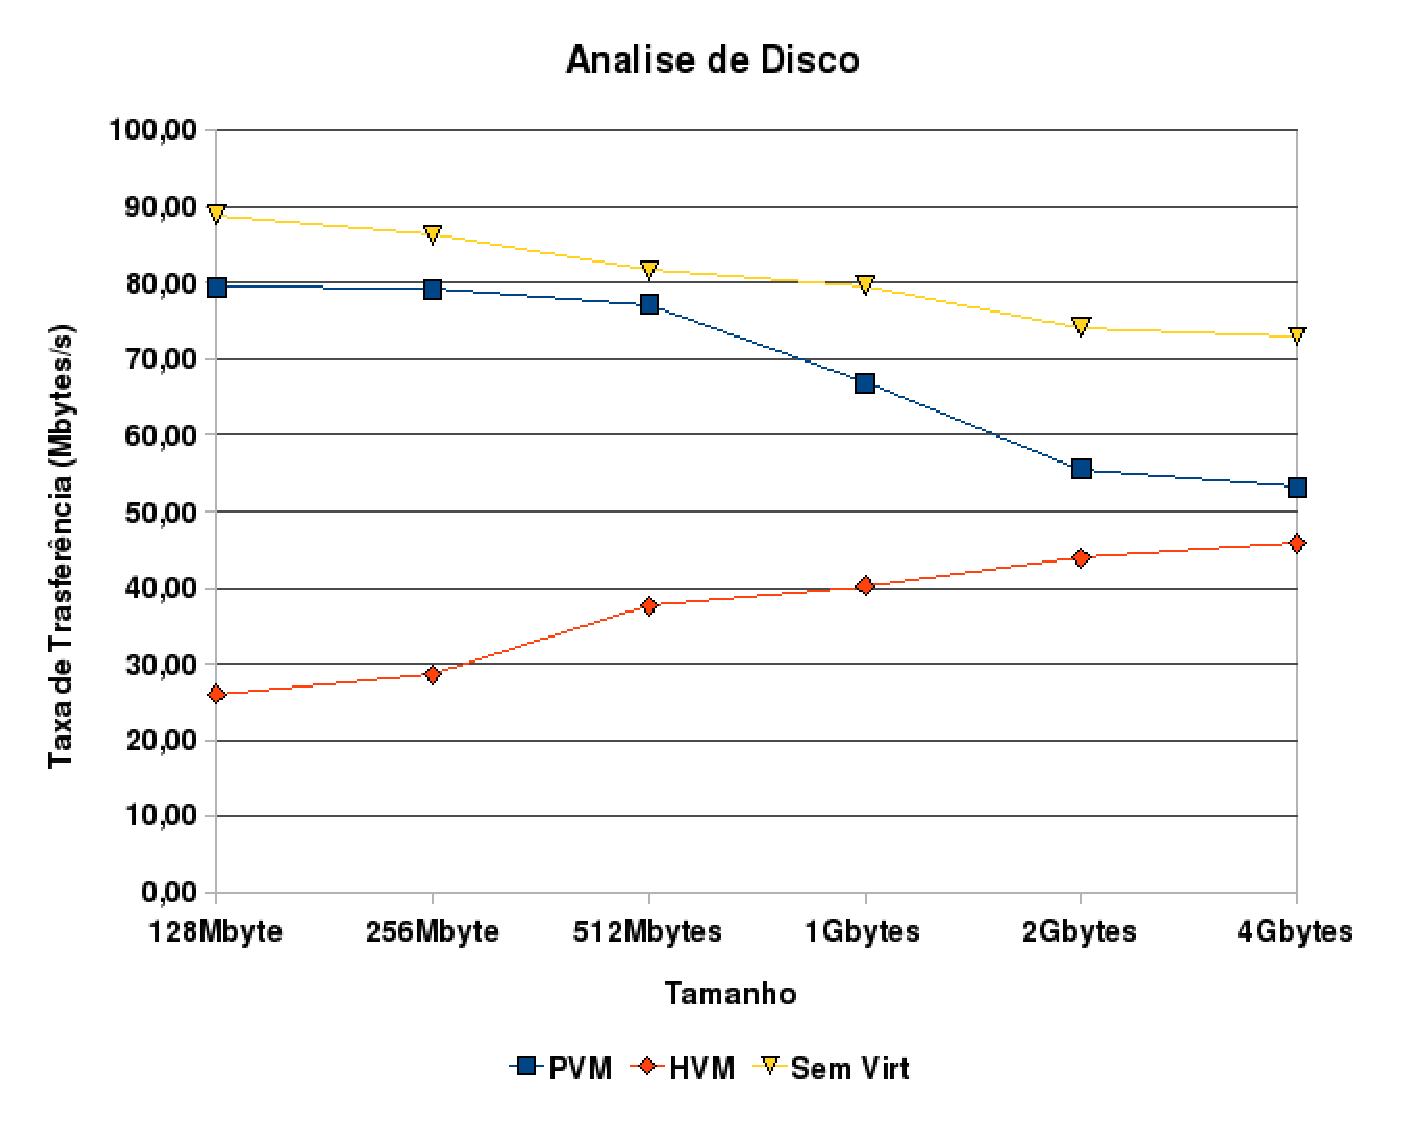
\includegraphics{img/disco_taxa.eps}}
\caption{Taxa de transferência de arquivos no disco em Mbytes/s}
\label{fig:disco_t}
\end{figure}

O segundo dado obtido pelo aplicativo é o tempo de transferência entre os arquivos,
mostrado na Figura \ref{fig:disco_tmp}, a qual confirma a maior sobrecarga
da máquina HVM e reforça o baixo impacto causado pela técnica de paravirtualização,
pois os tempos de transferência são similares aos da máquina real.

\begin{figure}[!htb]
\centering 
\resizebox{8.7cm}{!}{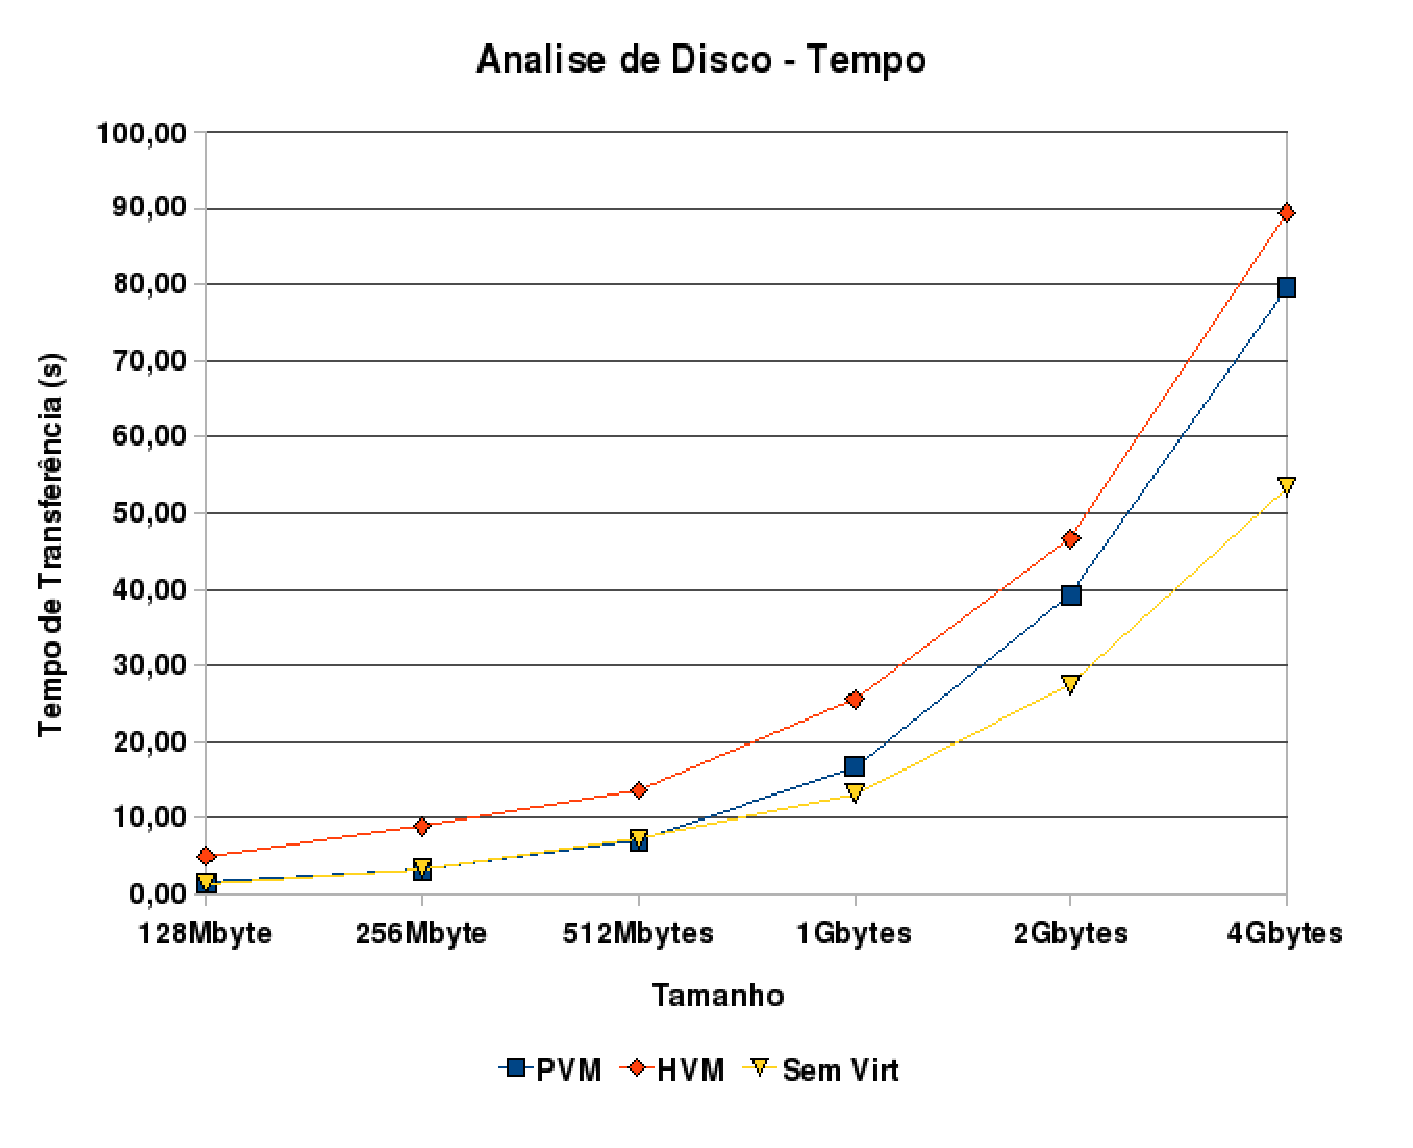
\includegraphics{img/disco_tmp.eps}}
\caption{Tempo de transferência de arquivos no disco em segundos}
\label{fig:disco_tmp}
\end{figure}

\subsection{Utilização de CPU}
As análises de CPU realizadas com o \textit{benchmark} Linpac-pc mostraram
resultados praticamente idênticos entre as tecnologias empregadas e a máquina
real, permanecendo em torno de 218,30 Mflops.

\subsection{Análise dos Resultados} 
Conforme já mencionado anteriormente, nestas análises foi possível verificar 
que embora uma MV HVM tenha acesso direto ao \kernel, sem interferência direta 
do MMV, a sobrecarga causada pelo \textit{firmware} na MV e o \textit{daemon}
no \hpv é consideravelmente grande face a máquinas PVM. A emulação dos dispositivos
de I/O prejudica consideravelmente o desempenho de rede e acesso a disco em 
máquinas virtuais HVM, as quais apresentam um desempenho inferior tanto para 
máquina real como para PVM, principalmente para mensagens e arquivos menores, 
nos quais o desempenho sem virtualização é significativamente maior.

Embora ambas as técnicas utilizadas mapeiem e reservem uma porção da memória para a 
MV, na virtualização de acesso a memória, o melhor desempenho da técnica de 
virtualização total é justificado pela diferença na forma como o \mmv implementa 
este acesso em relação as máquinas paravirtualizadas. As caracteristicas que 
proporcionam um melhor desempenho aos domínios HVM são o não compartilhamento de 
memória com as máquinas virtuais e a utilização de instruções que permitem um acesso
direto a mesma, diminuindo assim a sobrecarga sobre a virtualização de componente.

Com relação a utilização da CPU, o desempenho obtido foi praticamente o mesmo, 
apresentando mínimas variações nas medições, conforme a Tabela \ref{t:cv},
e uma diferença de 0,5 Mflops entre a MV HVM e as outras máquinas.


%------------------------------------------------------------------------- 
\section{Considerações Finais}\label{s:fim}
Neste trabalho analisou-se o desempenho das comunicações de rede entre máquinas não
virtuais e máquinas virtualizadas com as tecnologias de paravirtualização e 
virtualização total implementadas pelo \hpv Xen. 

De modo geral, a virtualização assistida por \hw oferecida pelo Xen deixa muito a 
desejar nos quesitos de comunicação de rede e acesso a disco, se comparada com a 
sua abordagem de  paravirtualização, a qual permanece como uma solução mais eficaz 
e com um menor impacto sobre o desempenho destes dispositivos. 

No entanto, se a necessidade de utilização de sistemas cujo \kernel não permite
modificações sobrepõem as necessidades de desempenho, é imperativo uso da técnica de
virtualização total, visto que a paravirtualização não permite a execução destes 
sistemas.

Assim, dependendo da abordagem utilizada, podem-se obter resultados de desempenho 
significativamente diferentes, que atrelados ao tipo de uso das MV e aos 
sistemas a serem utilizados, podem prover um embasamento para que administradores 
de sistemas e até mesmo usuários convencionais realizem uma opção entre utilizar ou
não a virtualização ou no caso de uso da mesma, qual tecnologia  melhor atende 
ao seus requisitos. 

Como trabalhos futuros, tem-se a intenção de comparar estas abordagens com a 
virtualização suportada pelo KVM -- \textit{Kernel-based Virtual Machine},
disponibilizado no \kernel Linux a partir da versão 2.6.20~\cite{kvm}.

%------------------------------------------------------------------------- 
%\nocite{ex1,ex2}
\bibliographystyle{conf/wscad_ieee}
\bibliography{ref-wscad}

\end{document}

%% <!-- Local IspellDict: brasileiro -->
%% <!-- Local Variables: -->
%% <!-- mode:flyspell -->
%% <!-- End: -->
